\section{Higgs Boson Phenomenology}\label{sec:higgs_pheno}

\subsection{Higgs Boson Production and Decay Modes}
In the SM, the Higgs boson directly couples to all particles except the gluon and photon, meaning that the Higgs boson can be produced in many different ways at the LHC, and can decay into a variety of final states. In this section, the main production and decay modes of the Higgs boson at the LHC are catalogued, and a discussion about the types of new physics that can be probed via each of them is begun. This is particularly relevant for the EFT interpretation in \cref{chap:eft} where that discussion will continue, and will also be useful for the di-Higgs search in \cref{chap:dihiggs}.

For proton-proton collisions at a center-of-mass energy of $\sqrt{s}=13\TeV$, the dominant production modes of the Higgs boson (those with the largest cross section) are gluon-gluon fusion (\ggH), vector boson fusion (\VBF), associated production with a vector boson (\VH), and associated production with a top quark-antiquark pair (\ttH). Further, subdominant production modes include single-top associated production (\tH), gluon-initiated associated production with a Z boson (\ggZH), and associated production with a bottom quark-antiquark pair (\bbH). Leading order diagrams for these processes are shown in \cref{fig:higgs_dominant_prod,fig:higgs_subdominant_prod} and their cross sections are provided in \cref{tab:higgs_xs}.

The Higgs boson decay modes can be categorized by whether they lead to a two-body final state, or a four-body final state. The two-body final states include decays to massive fermions, and decays to gluons or photons. Since the Higgs boson does not couple directly to gluons or photons, the decays to these particles proceed via loops of predominantly top quarks, where in \Hgg decays, loops of \PWpm bosons are also allowed. The LO Feynman diagrams for these decays are shown in \cref{fig:higgs_loop_decay}. The four-body decays arise from the decay of the Higgs boson to \WW or \ZZ, where the vector bosons further decay into leptons or quarks. The most common decay channels are \Hbb, \HWW, \Hgluglu, \Htautau, \Hcc, \HZZ, and \Hgg, and their branching fractions are shown in \cref{tab:higgs_brs}. 

\begin{table}
  \caption[Cross Sections for Higgs Boson Production Modes]{Standard Model predictions of the cross sections for different Higgs boson production modes in proton-proton collisions at $\sqrt{s}=13\TeV$ for $\mH=125$\GeV~\cite{LHCHiggsCrossSectionWorkingGroup:2016ypw}.}
  \begin{tabular}{cccccccccc}
    \toprule
    Production mode & \ggH & \VBF & \WH & \ZH & \bbH & \ttH & \ggZH & \tHq & \tHW \\ \midrule
    Cross section [$\pb\,$] & 48.6 & 3.78 & 1.37 & 0.761 & 0.528 & 0.507 & 0.123 & 0.074 &  0.015 \\ \bottomrule
    
  \end{tabular}\label{tab:higgs_xs}
\end{table}

\begin{figure}
  \centering
  \inputtikz{Figures/Theory/Higgs/ggh.tex}
  \inputtikz{Figures/Theory/Higgs/vh.tex}
  \inputtikz{Figures/Theory/Higgs/vbf.tex}
  \inputtikz{Figures/Theory/Higgs/tth.tex}
  \caption[LO Feynman Diagrams for the Dominant Higgs Boson Production Modes]{LO Feynman diagrams for the dominant production modes of the Higgs boson in proton-proton collisions at $\sqrt{s}=13\TeV$. From left to right: gluon-gluon fusion (\ggH), associated production with a vector boson (\VH), vector boson fusion (\VBF), and associated production with a top quark-antiquark pair (\ttH).}\label{fig:higgs_dominant_prod}
\end{figure}

\begin{figure}
  \centering
  \inputtikz{Figures/Theory/Higgs/ggzh.tex}
  \inputtikz{Figures/Theory/Higgs/thq.tex}
  \inputtikz{Figures/Theory/Higgs/thw.tex}
  \inputtikz{Figures/Theory/Higgs/bbh.tex}
  \caption[LO Feynman Diagrams for the Subdominant Higgs Boson Production Modes]{LO Feynman diagrams for the subdominant production modes of the Higgs boson in proton-proton collisions at $\sqrt{s}=13\TeV$. From left to right: gluon-initiated associated production with a Z boson (\ggZH), single-top associated production with a quark (\tHq), single-top associated production with a \PW boson (\tHW), and associated production with a bottom quark-antiquark pair (\bbH).}\label{fig:higgs_subdominant_prod}
\end{figure}

\begin{table}
  \centering
  \caption[Branching Fractions for Higgs Boson Decay Modes]{Branching fractions for the dominant Higgs boson decay modes at $\mH=125$\GeV~\cite{LHCHiggsCrossSectionWorkingGroup:2016ypw}.}
  \begin{tabular}{ccccccccc}
    \toprule
    Decay mode & $\Pqb\Pqb$ & \WW & $\Pg\Pg$ & $\tau\tau$ & $\Pqc\Pqc$ & \ZZ & $\gamma\gamma$ & Other \\ \midrule
    Branching fraction [\%] & 58.2 & 21.4 & 8.19 & 6.27 & 2.89 & 2.62 & 0.227 & 0.194 \\ \bottomrule
  \end{tabular}\label{tab:higgs_brs}
\end{table}

\begin{figure}
  \centering
  \inputtikz{Figures/Theory/Higgs/hgluglu.tex} \\
  \inputtikz{Figures/Theory/Higgs/hgg_w.tex}
  \inputtikz{Figures/Theory/Higgs/hgg_t.tex}
  \caption[LO Feynman Diagrams for \Hgluglu and \Hgg Decays]{LO Feynman diagrams for the decay of the Higgs boson to two gluons (top) or two photons (bottom).}\label{fig:higgs_loop_decay}
\end{figure}

\subsection{Simplified Template Cross Sections}\label{sec:stxs}

Measurements of the Higgs boson take several forms where the simplest measurement is perhaps of the inclusive production cross section of the Higgs boson. This is often presented as a signal strength, $\mu$, which is the ratio of the measured cross section to the SM prediction. A combination of CMS analyses of Higgs boson events from proton-proton collisions at $\sqrtS=13$\TeV, corresponding to an integrated luminosity of 138\fbinv, measured this signal strength to be $\mu = 1.014^{+0.055}_{-0.053}$~\cite{CMS-PAS-HIG-21-018}. This measurement is consistent with the SM ($\mu=1$) and therefore does not suggest any strong presence of new physics. However, if there was a large deviation, this measurement alone would not provide great insight into the \textit{type} of new physics that may be present. The discrepancy could be explained by a difference in any one of the production or decay modes. 

To gain a better understanding of the type of new physics that may be present, the Higgs boson is also studied in a more differential way. This is facilitated by the Simplified Template Cross Section (STXS) framework~\cite{LHCHiggsCrossSectionWorkingGroup:2016ypw}, which provides a common binning scheme to be used across decay channels. The binning scheme is designed to maximize sensitivity to BSM effects whilst remaining as model-independent as possible, allowing interpretations in a variety of new physics models such as an Effective Field Theory (EFT), which is the topic of \cref{chap:eft}. 

The STXS framework is divided into stages of progressively greater granularity. It begins with stage 0, with bins according to production mode only, where the grouping is slightly different to the production modes previously mentioned. This binning is shown in \cref{fig:stxs_stage0}. There are bins for the \ggH, \VBF, \ttH and \bbH modes, a \VH hadronic bin which is the \VH mode where the \PV boson decays hadronically, \WH and \ZH leptonic bins for where \PV boson decays leptonically, and a \tH bin which includes both the \tHq and \tHW modes. The \ZH leptonic bin is further split by whether the event was $\Pg\Pg$ or $\Pq\Pq$ initiated (\ggZH or \qqZH). Finally, an analysis can choose to merge any of the bins if there is not enough data to measure them separately. 

Results under the STXS framework can be presented in a number of ways. When making measurements in a single Higgs boson decay channel, the results are often presented as $\sigma_i \cdot \BR^f$, where $\sigma_i$ is a cross section corresponding to a particular STXS bin, and $\BR^f$ is the branching fraction for the given decay channel. In a combination of decay channels, the results may be presented as several sets of $\sigma_i \cdot \BR^f$, one for each decay channel, or as $\sigma_i \cdot \BR^{\PZ\PZ}$ and ratios of branching fractions, $\BR^f / \BR^{\PZ\PZ}$, where the \HZZ decay channel is arbitrarily chosen as the reference channel.

In the CMS combination mentioned previously~\cite{CMS-PAS-HIG-21-018}, results are given in terms of $\sigma_i \cdot \BR^{\PZ\PZ}$ and $\BR^f / \BR^{\PZ\PZ}$ for the stage 0 STXS where the \bbH bin is merged into the \ggH bin, and the \ggZH and \qqZH bins are also merged to form a single \ZH leptonic bin.  These results, shown in \cref{fig:stage0_measurement}, allow for deviations in specific production and/or decay modes to be highlighted. In this case, the measured cross sections in the \WH and \ZH leptonic modes are higher than their predictions, and there is a notable deviation for $\BR^{\PZ\gamma}/\BR^{\PZ\PZ}$, which together, suggest enhanced Higgs boson couplings to \PW and \PZ bosons. There is also an enhancement for \tH production, and a discrepancy for $\BR^{\Pqb\Pqb}/\BR^{\PZ\PZ}$. Overall, there is poor compatibility with the SM, corresponding to a p-value of 0.01.

\begin{figure}[p]
  \centering
  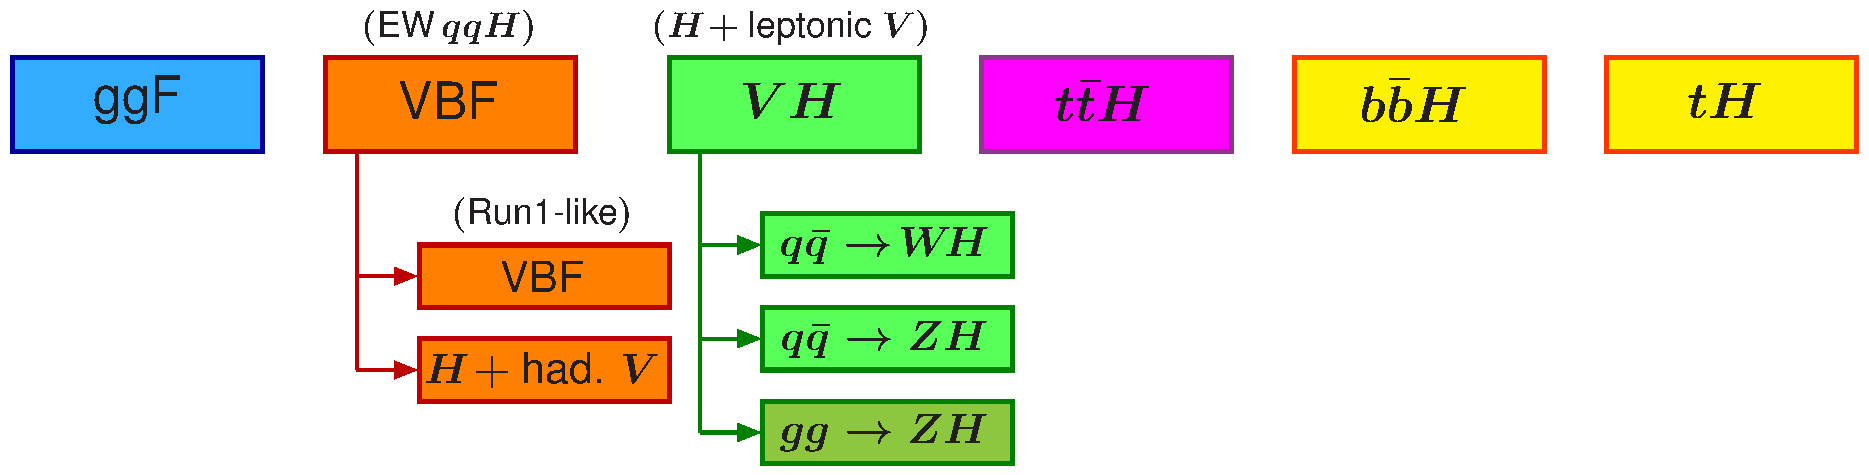
\includegraphics[width=\textwidth]{Figures/Theory/Higgs/STXS/simplifiedXS_stage0.pdf}
  \caption[Stage 0 Binning in the STXS]{Stage 0 binning in the STXS.}\label{fig:stxs_stage0}
\end{figure}

\begin{figure}[p]
  \centering
  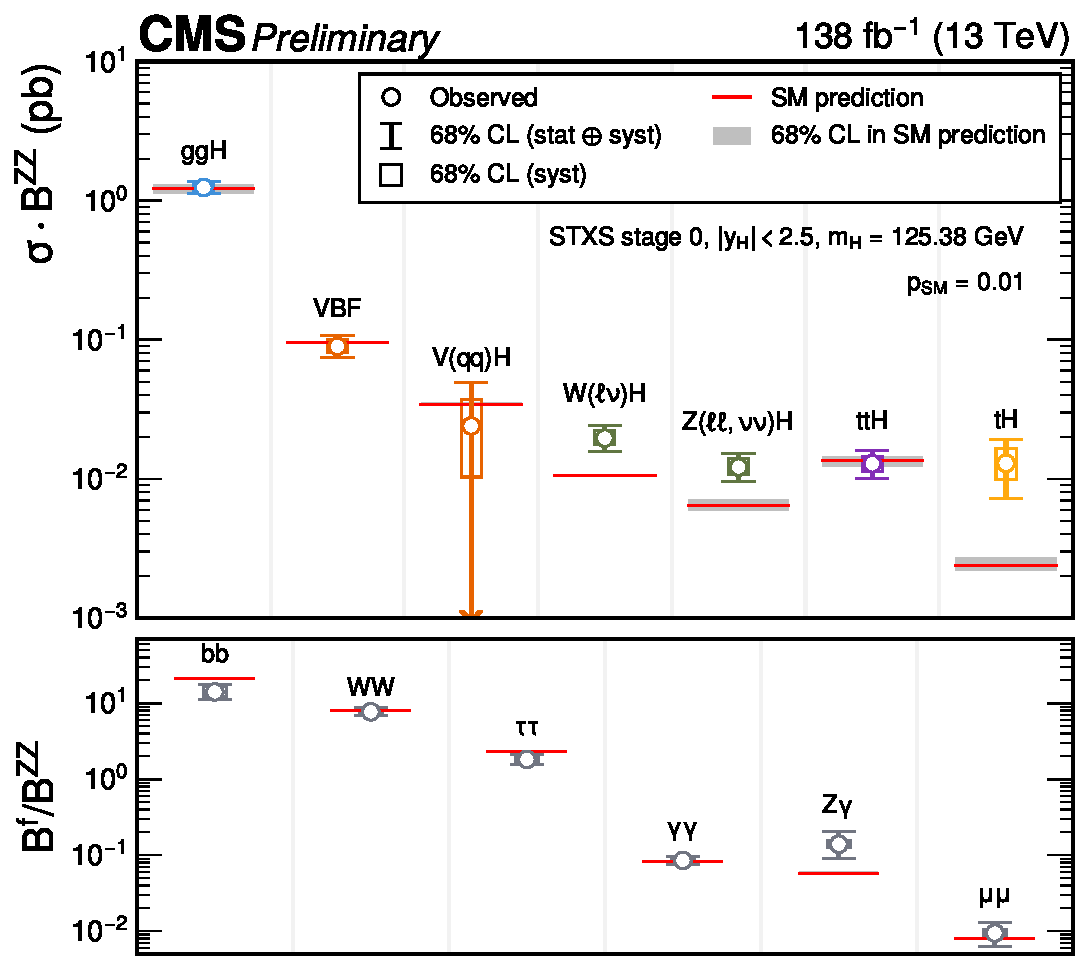
\includegraphics[width=0.8\textwidth]{Figures/Theory/Higgs/HIG-21-018-Figure_005-a.pdf}
  \caption[Measurements of the Stage 0 STXS]{STXS stage 0 cross sections and branching fraction ratios measured by the CMS experiment in a combination of Higgs boson decay channels in proton-proton collisions at $\sqrtS=13$\TeV corresponding to an integrated luminosity of 138\fbinv~\cite{CMS-PAS-HIG-21-018}. Theoretical uncertainties which affect the normalizations of the measured parameters are not included in the fit.}\label{fig:stage0_measurement}
\end{figure}

Additional information can be extracted by splitting the stage 0 bins further by e.g.\ the Higgs boson \pt, and this is where the later stages of the STXS come in. Schematics for the stage 1.2 binning are shown in \cref{fig:stxs_ggh,fig:stxs_vbf,fig:stxs_vh,fig:stxs_tth}. The variables used to split the bins, and the number of bins depends on the production mode. The stage 0 \ggH bin is split according to the Higgs boson transverse momentum, \ptH, the number of jets in the event, and in cases of $\geq 2$ jets, the invariant mass of the two leading jets, \mjj, and the transverse momentum of the Higgs boson and the two jets, \ptHjj. For $\ptH>200$\GeV, there is further splitting according to $\ptHj / \ptH$, where \ptHj is the transverse momentum of the Higgs boson and the leading jet. Excepting \ptHj, the stage 0 \qqH bin is split according to the same variables. The \VH bins are split by the transverse momentum of the vector boson, \ptV, and the number of jets in the event. The \ttH bin is split by \ptH only. Finally, the \bbH and \tH bins are not split further in stage 1.2 as there is limited experimental sensitivity to them.

\begin{figure}
  \centering
  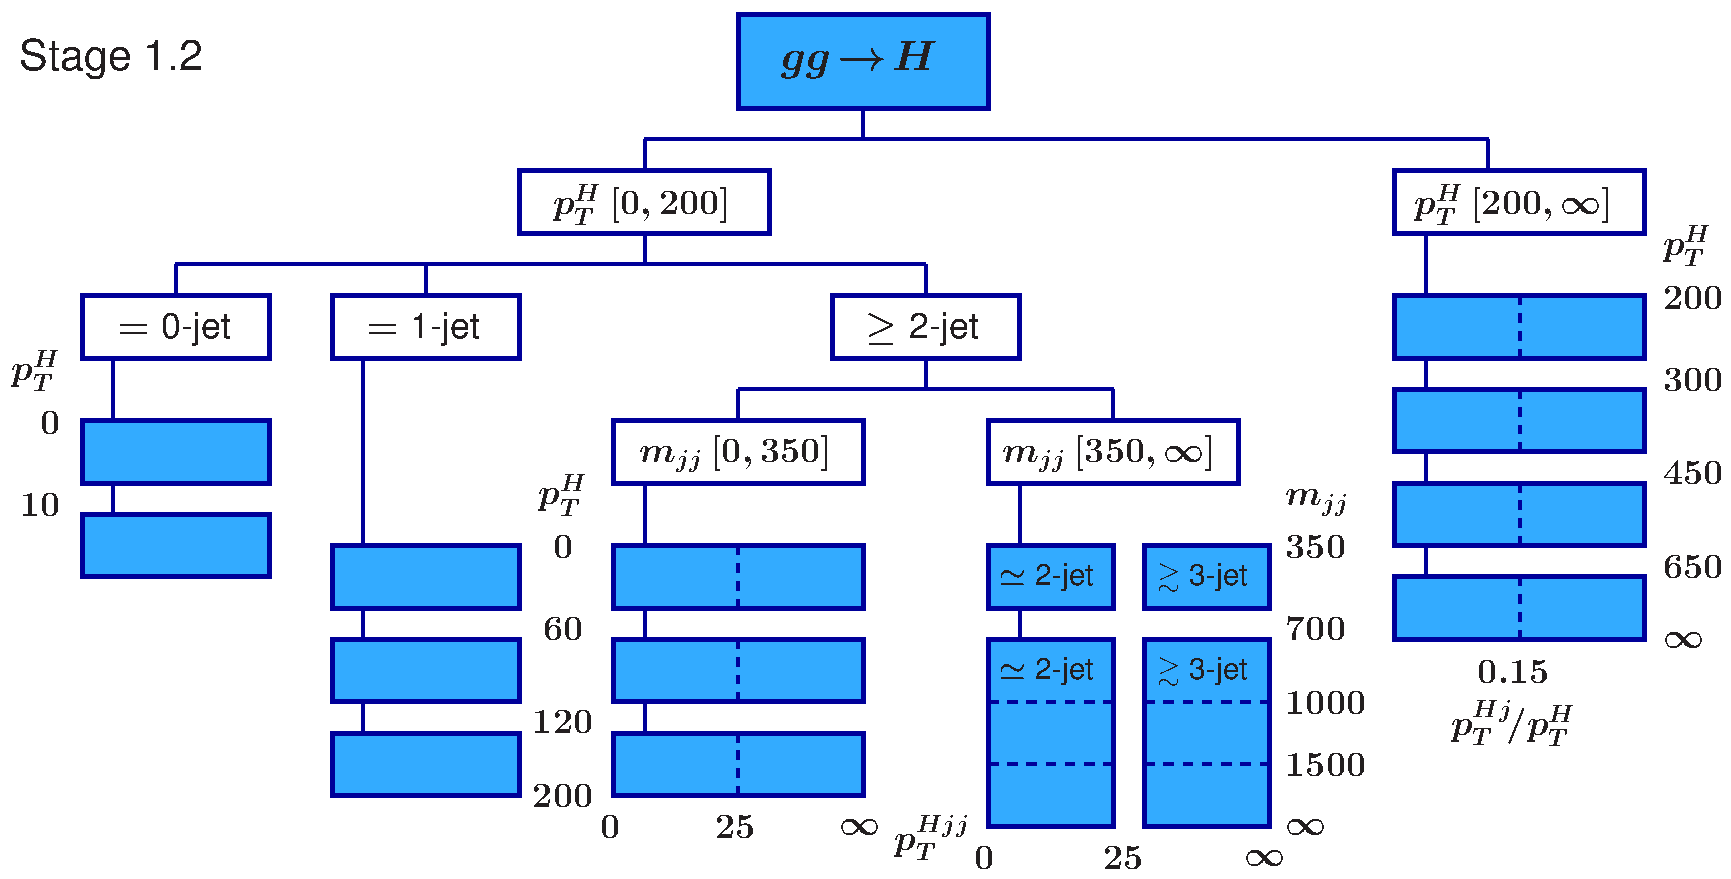
\includegraphics[width=\textwidth]{Figures/Theory/Higgs/STXS/simplifiedXS_ggF_1_2.pdf}
  \caption[Stage 1.2 \ggH Binning in the STXS]{Stage 1.2 binning for the \ggH production mode in the STXS.}\label{fig:stxs_ggh}
\end{figure}

\begin{figure}
  \centering
  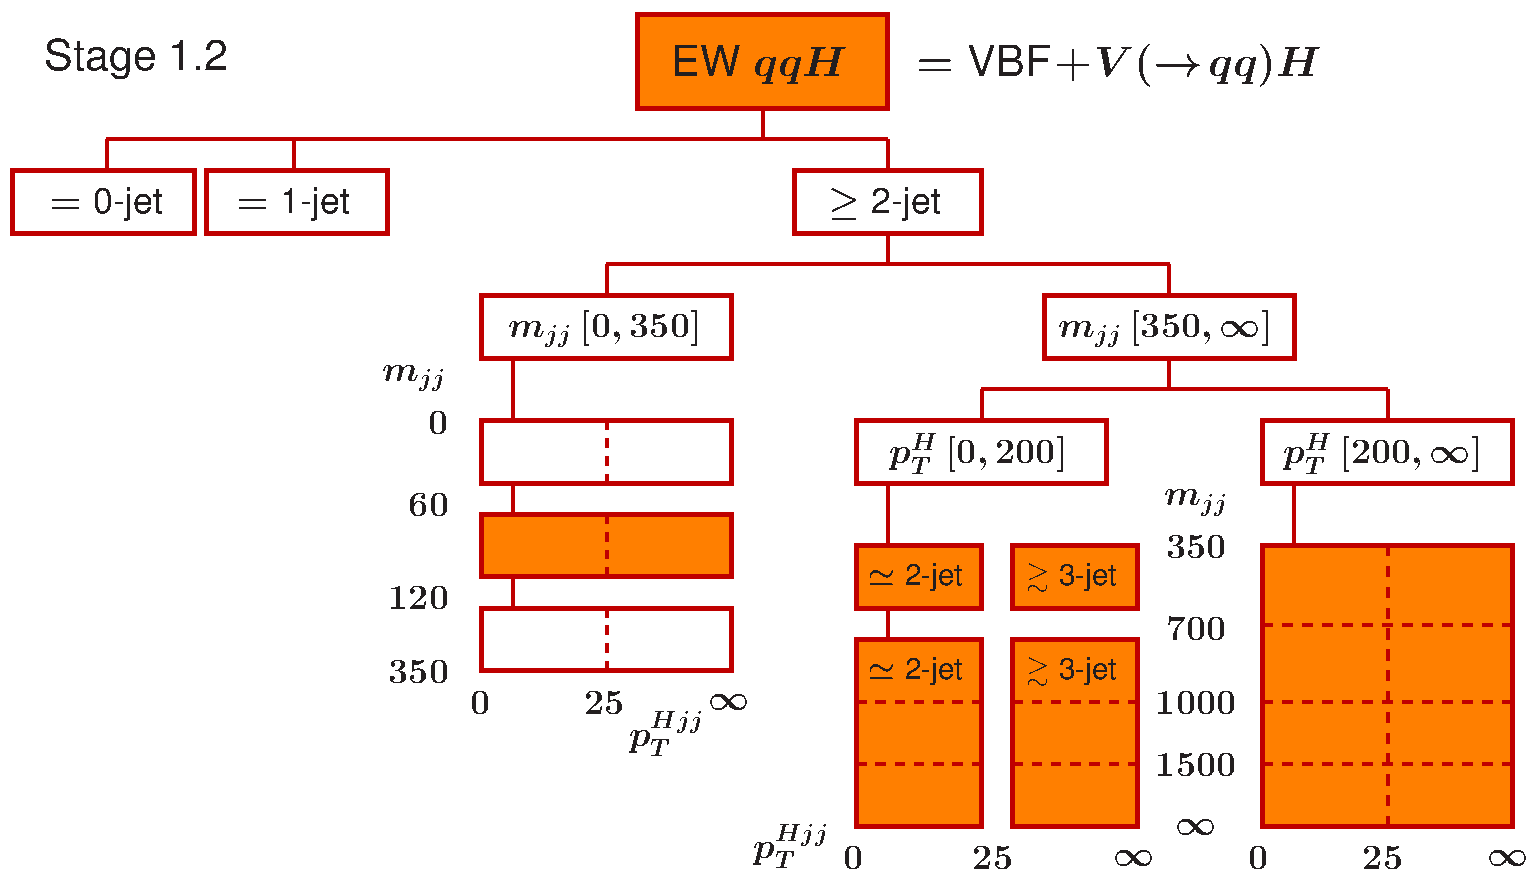
\includegraphics[width=0.8\textwidth]{Figures/Theory/Higgs/STXS/simplifiedXS_VBF_1_2.pdf}
  \caption[Stage 1.2 \VBF Binning in the STXS]{Stage 1.2 binning for the \qqH production mode in the STXS.}\label{fig:stxs_vbf}
\end{figure}

\begin{figure}
  \centering
  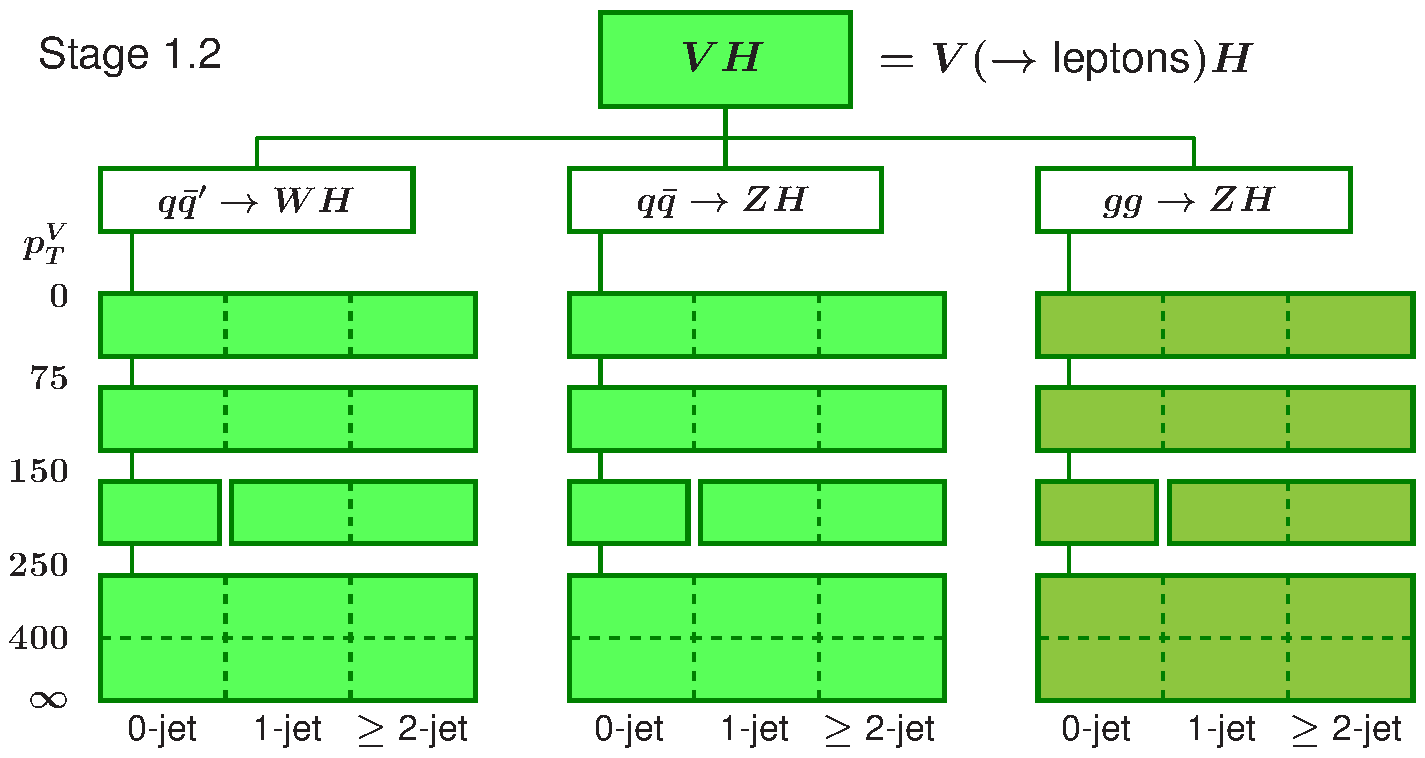
\includegraphics[width=0.8\textwidth]{Figures/Theory/Higgs/STXS/simplifiedXS_VH_1_2.pdf}
  \caption[Stage 1.2 \VH Binning in the STXS]{Stage 1.2 binning for the \VH leptonic production mode in the STXS.}\label{fig:stxs_vh}
\end{figure}

\begin{figure}
  \centering
  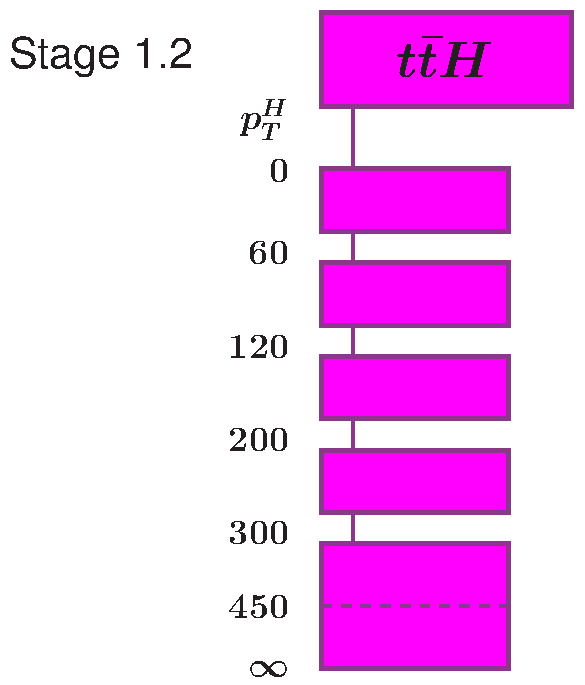
\includegraphics[width=0.3\textwidth]{Figures/Theory/Higgs/STXS/simplifiedXS_ttH_1_2.pdf}
  \caption[Stage 1.2 \ttH Binning in the STXS]{Stage 1.2 binning for the \ttH production mode in the STXS.}\label{fig:stxs_tth}
\end{figure}

The number of bins defined per production mode depends on the expected sensitivity, where \ggH, \qqH, \VH, and \ttH have 27, 24, 45, and 6 bins respectively where in \cref{fig:stxs_ggh,fig:stxs_vbf,fig:stxs_vh,fig:stxs_tth}, dashed lines indicate suggested places for bins to be merged. In the CMS combination~\cite{CMS-PAS-HIG-21-018}, a total of 32 bins were measured simultaneously: 13 for \ggH, 5 for \qqH, 4 for \WH leptonic, 4 for \ZH leptonic, 5 for \ttH, and a single bin for \tH. The results, in terms of $\sigma_i \cdot \BR^{\PZ\PZ}$ and $\BR^f / B^{\PZ\PZ}$, are shown in \cref{fig:stxs_stage1p2_results}. The compatibility with the SM is slightly better than the stage 0 results, with a p-value of 0.06. Now, in this stage 1.2 splitting, the \WH and \ZH disagreement can be identified as originating primarily by the $\ptV > 250$\GeV bins. 

\begin{figure}
  \centering
  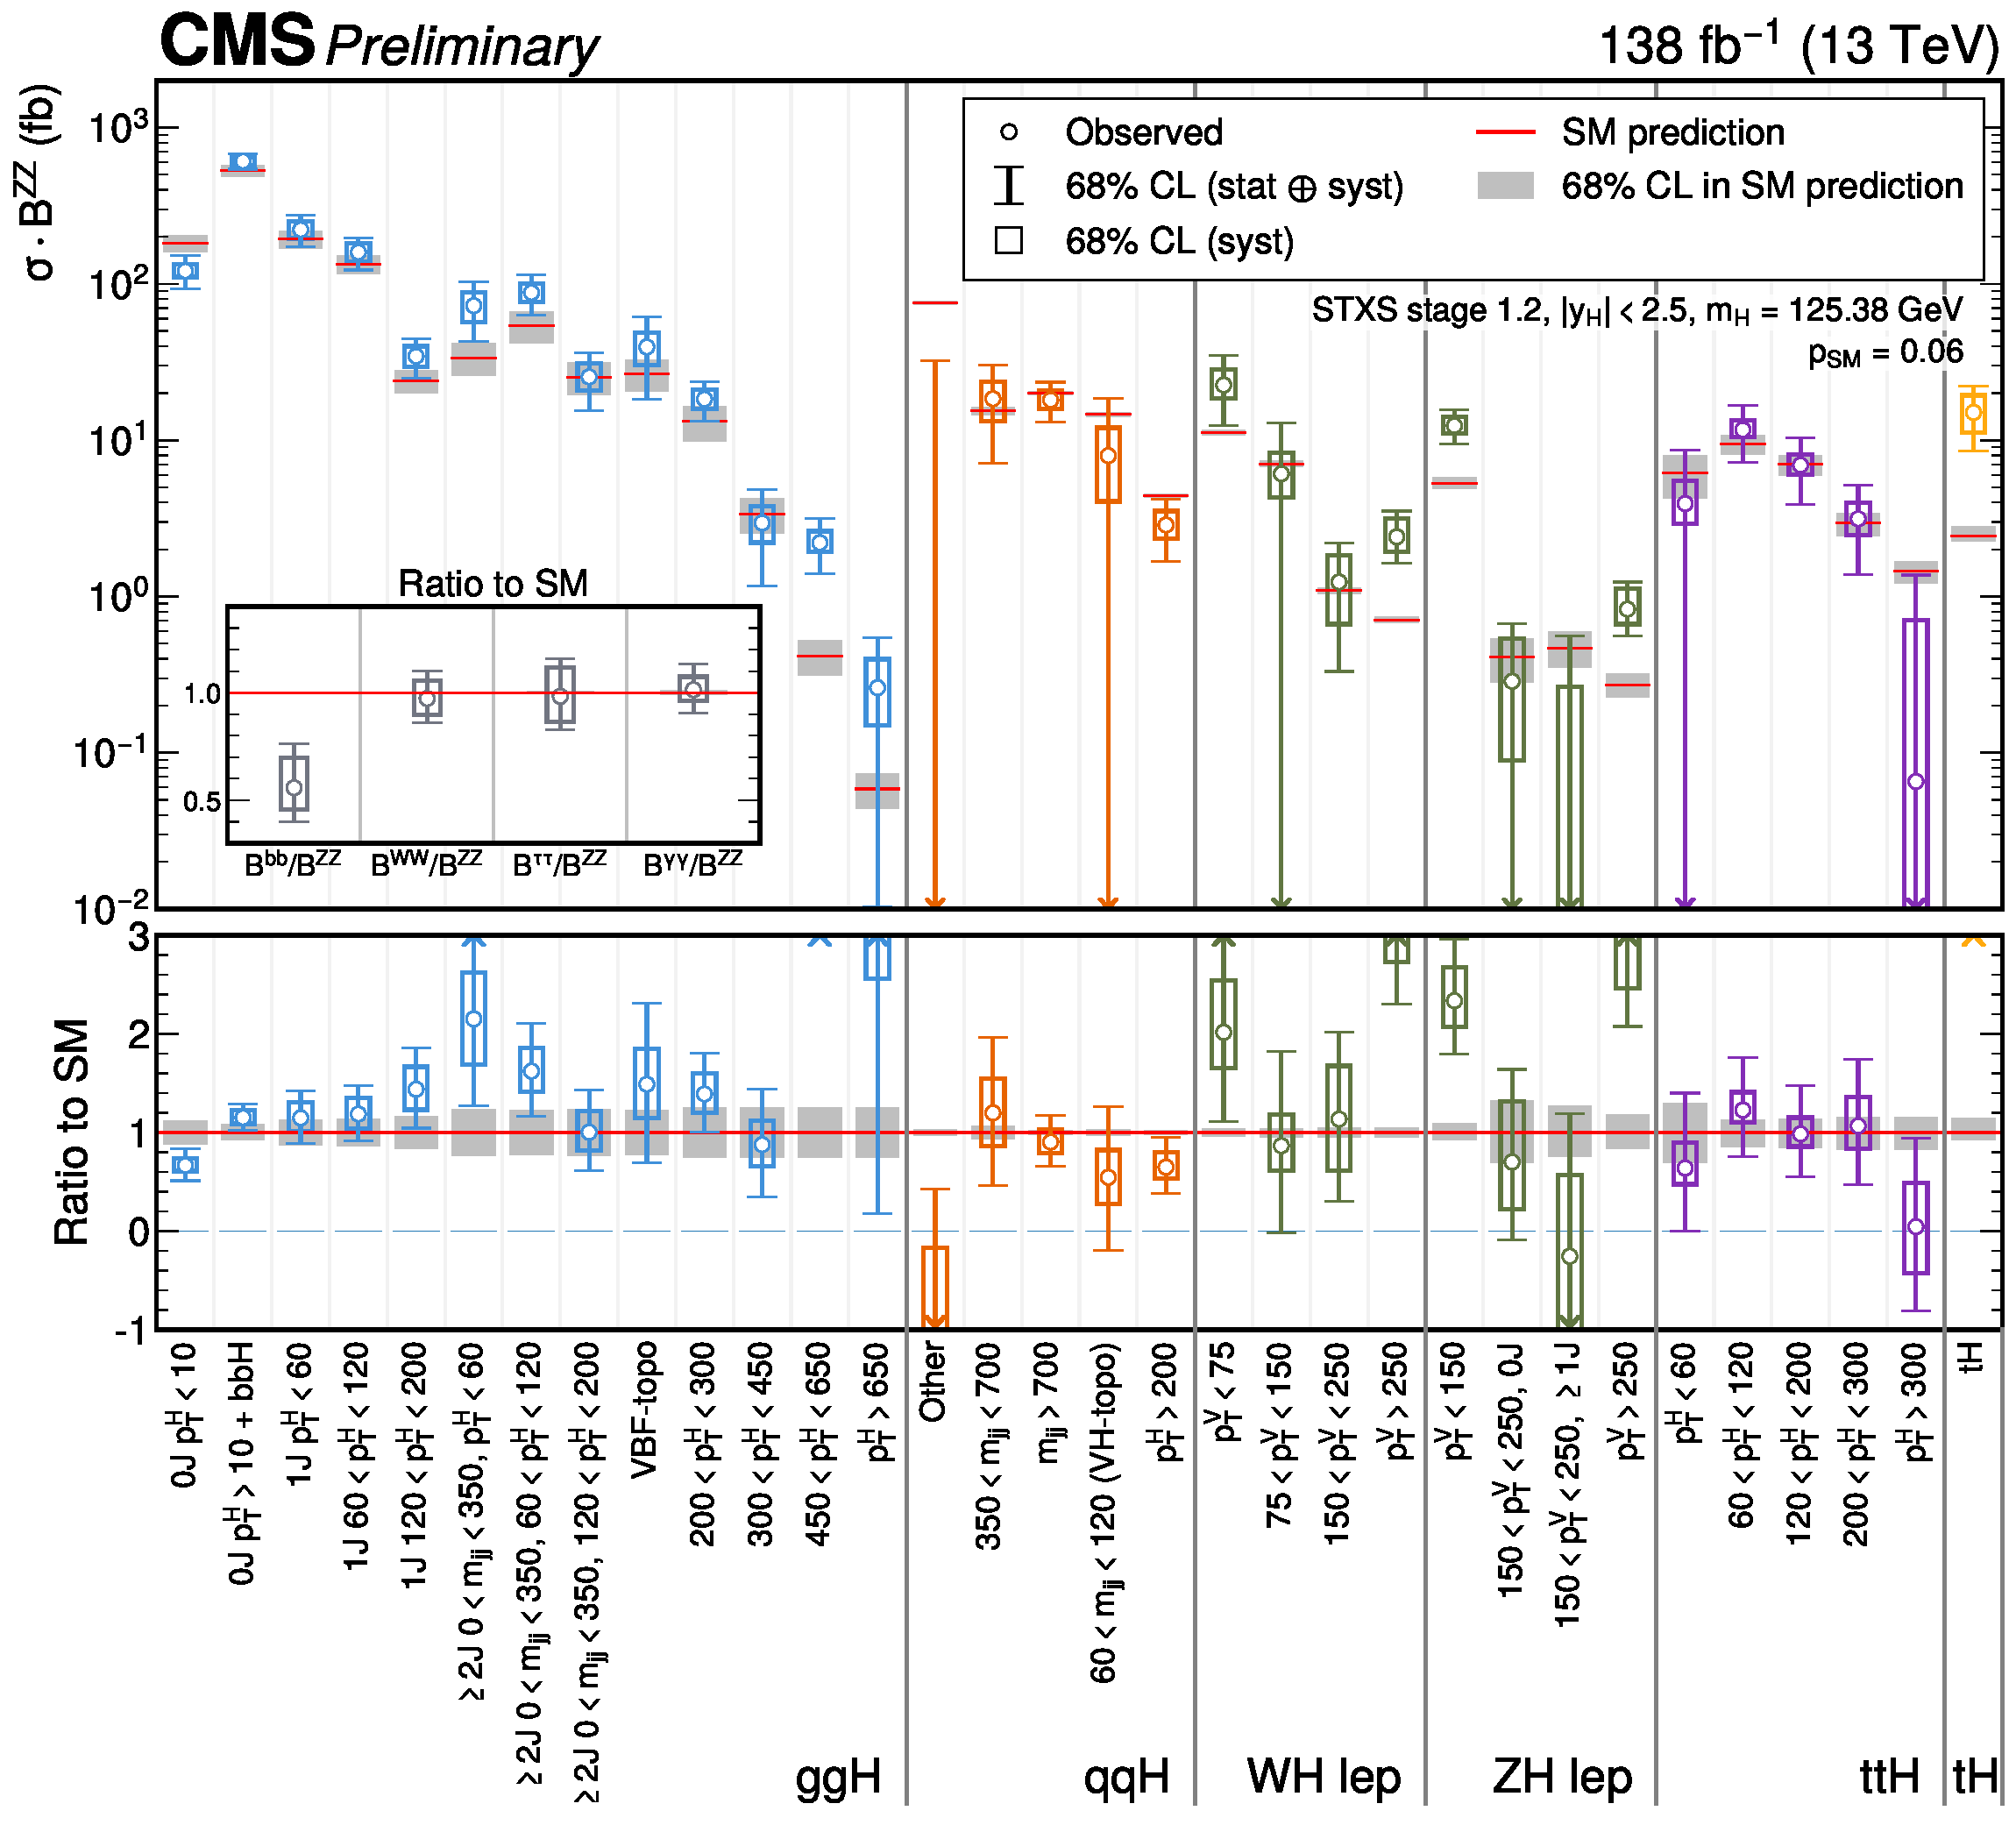
\includegraphics[width=\textwidth]{Figures/Theory/Higgs/HIG-21-018-Figure_006.pdf}
  \caption[Measurements of the Stage 1.2 STXS]{STXS stage 1.2 cross sections and branching fraction ratios measured by the CMS experiment in a combination of Higgs boson decay channels in proton-proton collisions at $\sqrtS=13$\TeV corresponding to an integrated luminosity of 138\fbinv~\cite{CMS-PAS-HIG-21-018}. Theoretical uncertainties which affect the normalizations of the measured parameters are not included in the fit. In cases where the best-fit values and/or 68\% CL intervals lie outside the range of the plot, their location (above or below) is indicated by arrows.}\label{fig:stxs_stage1p2_results}
\end{figure}

Finally, the results are also presented in terms of $\sigma_i \cdot \BR^f$ for every input decay channel as shown in \cref{fig:stxs_stage1p2_results_split}. Now, the origins of the disagreements in the cross sections can be identified from the individual decay channels and consistency checks can be performed. For example, enhancements in the high \ptV \WH leptonic bins are driven by the \Hbb, \HWW and \Htautau channels, and the excess for \tH is driven by the \Hgg channel which is the only channel with enough sensitivity to measure it separately from \ttH. 

A particular BSM theory can be confronted with these results by parameterizing the cross sections and branching fractions in terms of the theory's parameters, and then performing a fit to the data to place constraints on the theory parameters. This CMS combination does this with an Effective Field Theory (EFT), specifically the Standard Model EFT (SMEFT). The theoretical details underpinning this interpretation is discussed in \cref{sec:EFT} and the derivation of the SMEFT parameterization and the final results are discussed in \cref{chap:eft}.

\begin{landscape}
  \begin{figure}
    \centering
    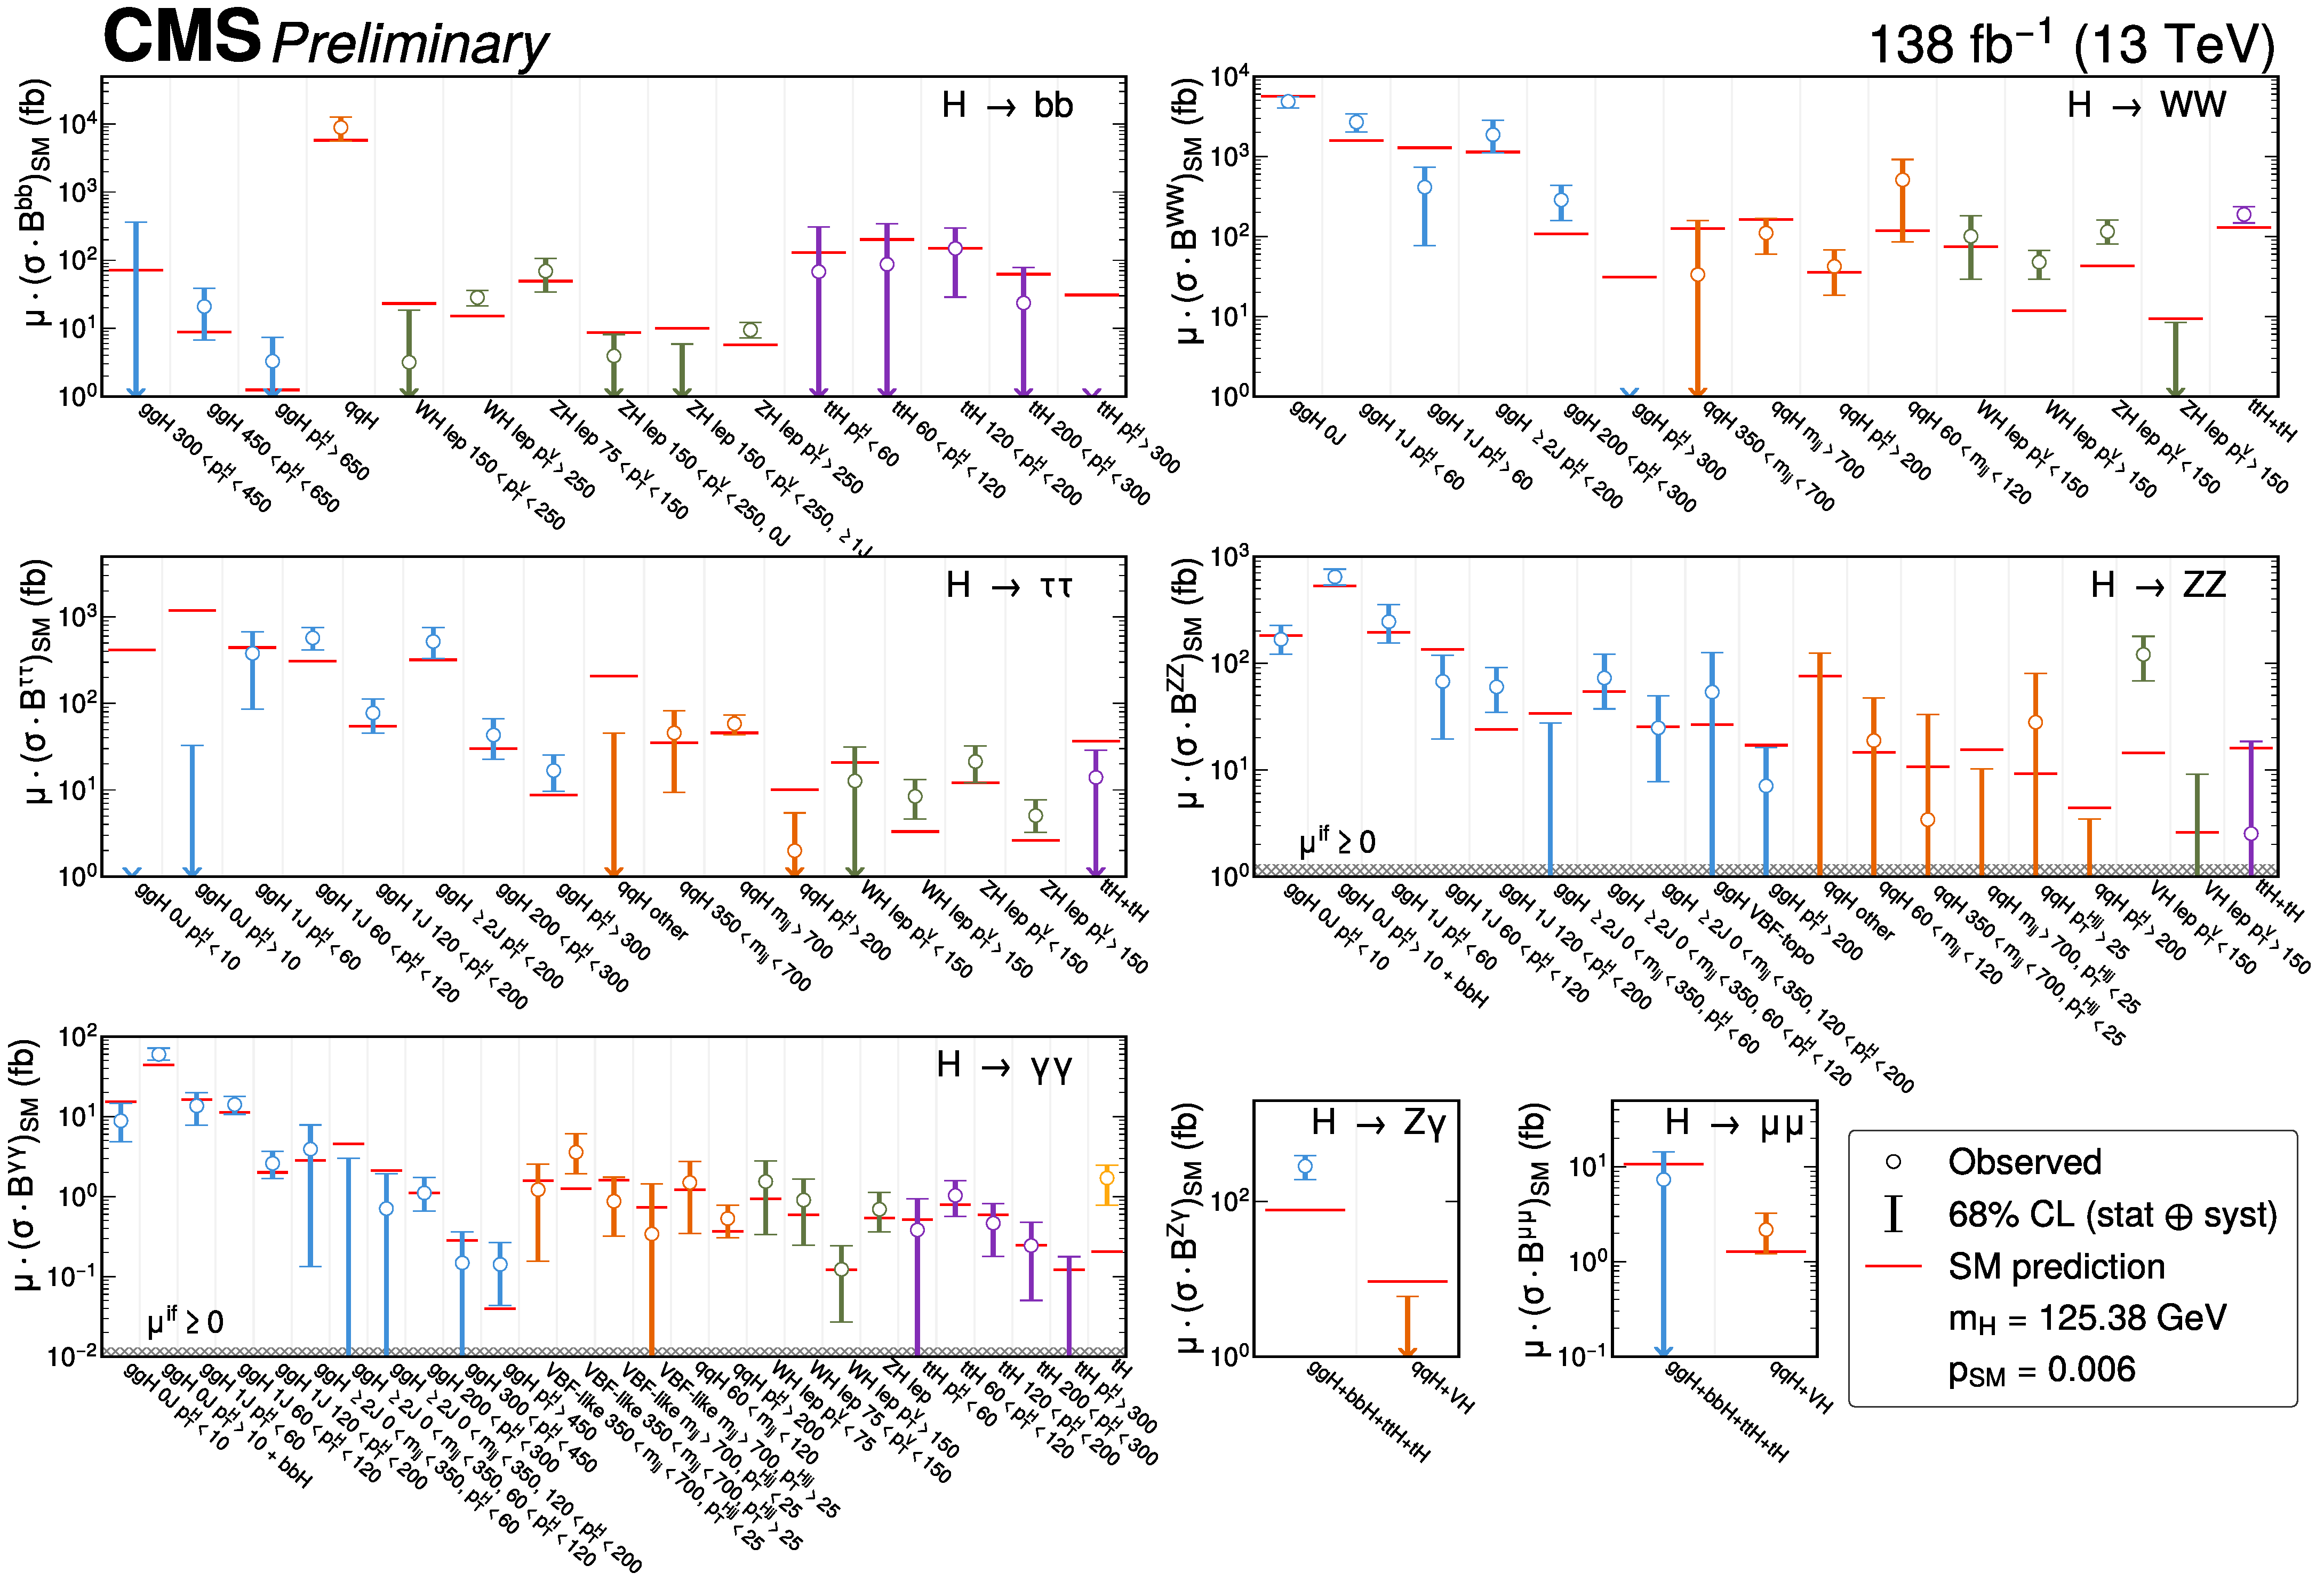
\includegraphics[width=0.9\pagewidth]{Figures/Theory/Higgs/HIG-21-018-Figure_008.pdf}
    \caption[Measurements of the Stage 1.2 STXS Split by Decay Channel]{STXS stage 1.2 cross section times branching fractions measured by the CMS experiment in a combination of Higgs boson decay channels in proton-proton collisions at $\sqrtS=13$\TeV corresponding to an integrated luminosity of 138\fbinv~\cite{CMS-PAS-HIG-21-018}. Theoretical uncertainties which affect the normalizations of the measured parameters are not included in the fit. In cases where the best-fit values and/or 68\% CL intervals lie outside the range of the plot, their location (above or below) is indicated by arrows. In the \Hgg and \HZZ decay channels, the results are constrained to be positive as indicated by the hatched grey lines.}\label{fig:stxs_stage1p2_results_split}
  \end{figure}
\end{landscape}